\documentclass[10pt]{article}
\usepackage[utf8]{inputenc}
\usepackage[T1]{fontenc}
\usepackage{graphicx}
\usepackage{appendix}
\usepackage[french]{babel}
\usepackage{fancyhdr}
\usepackage{geometry}
\geometry{hmargin=3cm,vmargin=3.5cm}
\usepackage{enumitem}
\usepackage{listings}
\usepackage{subcaption}
\usepackage{amsmath}
\usepackage{animate}
\graphicspath{{./img/}}
\lstset{ %
  backgroundcolor=\color{white},   % choose the background color; you must add \usepackage{color} or \usepackage{xcolor}
  basicstyle=\small,               % the size of the fonts that are used for the code
  breakatwhitespace=false,         % sets if automatic breaks should only happen at whitespace
  breaklines=true,                 % sets automatic line breaking
  captionpos=b,                    % sets the caption-position to bottom
  commentstyle=\color{blue},      % comment style
  escapeinside={\%*}{*)},          % if you want to add LaTeX within your code
  extendedchars=true,              % lets you use non-ASCII characters; for 8-bits encodings only, does not work with UTF-8
  frame=single,                    % adds a frame around the code
  keepspaces=true,                 % keeps spaces in text, useful for keeping indentation of code (possibly needs columns=flexible)
%  keywordstyle=\color{blue},       % keyword style
  language=C,                    % the language of the code
  numbers=left,                    % where to put the line-numbers; possible values are (none, left, right)
  numbersep=5pt,                   % how far the line-numbers are from the code
  numberstyle=\tiny\color{black},  % the style that is used for the line-numbers
  rulecolor=\color{black},         % if not set, the frame-color may be changed on line-breaks within not-black text (e.g. comments (green here))
  showspaces=false,                % show spaces everywhere adding particular underscores; it overrides 'showstringspaces'
  showstringspaces=false,          % underline spaces within strings only
  showtabs=false,                  % show tabs within strings adding particular underscores
  stepnumber=1,                    % the step between two line-numbers. If it's 1, each line will be numbered
  tabsize=2,                       % sets default tabsize to 2 spaces
}
\usepackage{hyperref}
\hypersetup{colorlinks=true}

\pagestyle{fancy}

\renewcommand{\sectionmark}[1]{ \markright{#1}{} }

\lhead{}
\rhead{}
\lfoot{ENSEIRB-MATMECA}
\rfoot{PRCD}
\renewcommand{\headrulewidth}{0.pt}
\renewcommand{\footrulewidth}{0.4pt}


\begin{document}
%\tableofcontents
%\newpage

\thispagestyle{empty}


%\begin{center}
%\includegraphics{enseirb_inp.png}
%\end{center}
%
%\vspace{\stretch{1}}
\hrule
\begin{flushleft}
\Huge{\textbf{Projet PG305}}\\
\textit{Craquage de mot de passe}
\end{flushleft}
\begin{flushright}
\huge\textbf{Rapport}\\
\end{flushright}
\hrule

\vspace{80pt}
\noindent\textbf{Élève :}
\emph{Aurélien Falco, Alexandre Honorat}\\
\\
\noindent\textbf{Responsable :}
\emph{Olivier Coulaud}\\


\vspace{60pt}
\normalsize
\begin{center}
  Troisième année, filière informatique, option PRCD\\
  Date : \today\\
  Enseirb-Matmeca
\end{center}
\vspace{50pt}

\section*{Introduction} % (fold)
\addcontentsline{toc}{section}{Introduction}
\label{sec:introduction}
Le but du projet était d'implémenter une recherche de mot de passe par force brute, répartie sur plusieurs processus. Dans ces processus la charge serait sur plusieurs threads OpenMP.


\newpage

\section{Recherche distribuée de mot de passe} % (fold)
\label{sec:recherche_de_mot_de_passe}

La recherche de mot de passe, étant effectuée par force brute, le fonctionnement du programme est très simple : le maître génère au début un certain nombre de tâches -- intervalles de mot de passes à tester -- puis envoie ces tâches aux esclaves qui en demandent. Cette section détaille plus précisément comment les communications s'effectuent entre le processus maître et les esclaves, jusqu'à la terminaison de tous.

\subsection{Directives de l'énoncé} % (fold)
\label{sub:enonce}

Le programme effectue une recherche de mot de passe par force brute. L'utilisateur lance tout d'abord un programme appelé master (maître). Celui-ci lance $p-1$ processus appelés slave (esclave). Chaque processus esclave lance à son tour $t+1$ \emph{threads}. Parmi ces \emph{threads}, un servira uniquement aux communications avec le maître et les autres effectueront des tâches. 

Le programme peut terminer de deux façons différentes :
\begin{itemize}
	\item Soit un des \emph{threads} de travail trouve le mot de passe. Dans ce cas, l'esclave correspondant envoie le mot de passe au maître. Ce dernier affiche le mot de passe, et ne donne plus de nouvelles tâches aux autres esclaves et termine.
	\item Soit personne ne trouve le mot de passe (mot plus long que la taille maximum donnée). Le maître attend que les esclaves terminent toutes les tâches et affiche que le mot de passe n'a pas été trouvé.
\end{itemize}

Les communications doivent être recouvertes par des calculs. Ainsi, un esclave demandera du travail bien avant d'avoir terminé son intervalle de recherche courant. En pratique, le \emph{thread} de communication demande une nouvelle tâche dès que sa pile locale contient moins de tâches que son nombre de \emph{threaads} de calcul. Si jamais les tâches ne sont pas arrivées à temps, les \emph{threads} de calculs s'endorment jusqu'à ce qu'une nouvelle tâche arrive. Il sont alors réveillés par le \emph{thread} de communication. Cette attente passive est réalisée grâce à l'utilisation de sémaphores. Notons que le \emph{thread} de communication fonctionne en attente active.

\subsection{Communications} % (fold)
\label{sub:communication}

Les \emph{threads} de communication respectivement du maître et de l'esclave s'échangent les même types de messages, mais ne font pas les mêmes actions en réponse. Ils sont ici représentés par les automates associés, figure \ref{fig:master} et \ref{fig:slave}. Les messages échangés peuvent être des différents types -- ou \emph{tag} suivants :
\begin{itemize}
\item \textbf{ASK} : un esclave demande une tâche supplémentaire au maître.
\item \textbf{END} : le maître signifie à un esclave que le mot de passe a été trouvé et qu'il doit terminer, en réponse à un \textbf{ASK}.
\item \textbf{INTER} : le maître envoie une tâche à un esclave, ou bien un esclave lui envoie le mot de passe. 
\item \textbf{FINISH} : le maître n'a plus de tâche à distribuer, en réponse à un \textbf{ASK}.
\item \textbf{NOTHING} : l'esclave a terminé et n'a pas trouvé de mot de passe, il en informe le maître.
\end{itemize}

\begin{figure}[h!]
\centering
\includegraphics[width=\textwidth]{automat-master}
\caption{Automate du maître}
\label{fig:master}
\end{figure}


\begin{figure}[h!]
\centering
\includegraphics[width=\textwidth]{automat-slave}
\caption{Automate de l'esclave}
\label{fig:slave}
\end{figure}

\section{Choix d'implémentation} % (fold)
\label{sec:impl}

Les fonctions des deux programmes -- maître et esclave -- sont peu nombreuses : chacun des deux possède une fonction de communication, le maître possède une fonction pour répartir les mots de passes, l'esclave une pour les vérifier.

\subsection{Demande de tâche} % (fold)

En pratique, le \emph{thread} de communication demande une nouvelle tâche dès que sa pile locale contient moins de tâches que son nombre de \emph{threaads} de calcul. Si jamais les tâches ne sont pas arrivées à temps, les \emph{threads} de calculs s'endorment jusqu'à ce qu'une nouvelle tâche arrive. Il sont alors réveillés par le \emph{thread} de communication. Cette attente passive est réalisée grâce à l'utilisation de sémaphores. Notons que le \emph{thread} de communication fonctionne en attente active.

\subsection{Représentation du mot de passe}

Le mot de passe peut avoir ses caractères compris dans l'ensemble de l'alphabet \textsf{ASCII}. Les chaînes de caractères en \textsf{C} sont des tableaux commençant à l'indice $0$ et terminées à droite par un élément nul. Il n'est donc pas aisé de les étendre à gauche, ce qui es la manière la plus simple de considérer l'ordre de création les mots de passe : généralement pour passer aux mots de la longueur supérieure, une lettre est ajoutée à sa gauche. Pour pallier ce problème, nous déterminons le mot miroir du mot de passe, et nous étendons au fur et à mesure du calcul les mots par la droite. C'est ainsi le mot de passe miroir qui est trouvé, puis renversé lors de l'affichage de la solution.

Par ailleurs les considérations mathématiques pour passer d'un mot à son successeur -- les tâches n'étant que des intervalles de mots à tester : le premier mot puis une longueur donnée -- rendent compliquées l'utilisation directes des caractères de type \texttt{char} du mot de passe en entrée. Il est beaucoup plus simple de considérer que les lettres vont de $1$ au nombre de lettres de l'alphabet. Le zéro est quand à lui toujours réservé à la fin du mot.


\subsection{\'Eclatement des intervalles}

Un intervalle est composé de deux éléments : un mot de départ et le nombre de mots à vérifier. Ainsi chaque \emph{thread} peut vérifier tout un intervalle en utilisant à chaque itération la fonction calculant le mot suivant. La taille de ces intervalles est une constante définie dans le fichier d'en-têtes. Une taille arbitrairement grande a été choisie afin de ne pas surcharger le maître en communications. La terminaison du programme n'étant pas directe et se prduisant uniquement lorsque le maître n'a plus donné de nouvelles tâches aux esclaves, impose donc que tous les \emph{threads} de calcul ont terminé leur tâche courante avant la terminaison générale. Il convient donc de ne pas non plus mettre une valeur trop importante. Actuellement $100000$ mots sont testés par tâche.

L'ordre utilisé pour organiser la liste des mots à tester est ici lexicographique par taille, c'est-à-dire que nous comparons d'abord tous les mots d'une certaine longueur, dans l'ordre lexicographique, pour ensuite pouvoir passer aux mots comportant une lettre de plus. Le calcul du mot suivant, et sa version étendue du $\mathnormal{n}$-ième mot suivant, est un algorithme assez abscons, dont le fonctionnement n'est pas utile dans le cadre de ce projet.

Notons enfin que le calcul de tous les intervalles est effectué séquentiellement par le maître, avant le commencement des communications. Une voie possible d'amélioration est de commencer les communications dès le début afin de limiter la latence que cela induit. Toutefois le temps de création de ces intervalles reste bien inférieur au temps de calcul, et l'économie ne se ressentirait pas beaucoup.

\subsection{Accès à la pile de tâches}

Chaque esclave possède un certain nombre de tâches de réserver pour éviter la famine d'un de ses \emph{threads}, celles-ci sont stockées dans une pile -- ou plutôt liste doublement chaînée -- de l'implémentation \textsf{CCAN}. La pile des tâches est partagée entre les différents \emph{threads} de travail et celui de communication ; il convient donc de protéger l'accès. Pour cela les sections critiques d'accès à la pile sont encadrées par un \emph{pragma OpenMP} empêchant tout problème du à la concurrence -- voir l'exemple \ref{critical}. Ainsi, chaque \emph{thread} peut retirer une tâche de la file et l'exécuter sans crainte de dédoubler un travail, puisqu'il est forcément seul quand il arrive dans cette section. 

\begin{figure}
\begin{lstlisting}
	#pragma omp critical
	{
	  if( NOT list_empty( task_list ){
	    task_to_deal_with = pop( task_list );
	  }
	}
\end{lstlisting}
\caption{Section critique qui permet de récupérer une tâche}
\label{critical}
\end{figure}

\subsection{Parallèlisation des tests}

Chaque esclave possède plusieurs \emph{threads} exécutant autant de tâches en parallèle. Ces tâches sont totalement indépendantes puisqu'elles requièrent uniquement la lecture du véritable mot de passe pour s'y comparer, la parallèlisation est donc très aisée et est réalisée via \textsf{OpenMP}. D'abord le nombre de \emph{threads} en argument est spécifié à la bibliothèque d'\textsf{OpenMP}, ensuite une section est déclarée parallèle puis, si l'identifiant du \emph{thread} est zéro alors celui-ci s'occupe des communications, sinon -- donc tous les autres identifiants -- il exécute la fonction de calcul d'une tâche.

\section{Exécution \& tests} % (fold)
\label{sec:execution}

A l'exécution l'utilisateur peut passer certains paramètres au programme. Ceux-ci sont les suivants :
\begin{itemize}
	\item $p$ : nombre de processus total. $p-1$ esclaves seront créés ;
	\item $t$ : nombre de threads de travail. Au total, $t+1$ threads sont créés, en comptant le thread de communication ;
	\item $r$ : longueur maximum des mots à vérifier ;
	\item $m$ : le mot de passe.
	\item $c$ : le chemin de l'exécutable \og slave\fg .
\end{itemize}

Il est ainsi possible de changer facilement les paramètres du programme entre deux exécutions, ce qui nous a permis de le tester pour un certain nombre de cas. \`A noter que le programme retourne une erreur si les paramètres ne sont pas cohérents (par exemple si une lettre du mot de passe n'est pas dans l'alphabet donné).


\section{Performances} % (fold)
\label{sec:perf}

Pour les performances, nous avons créé un script qui nous permet de lancer des jobs sur la machine Plafrim de l'Inria. Le graphe de la figure \ref{fig:graph_procs} montre les résultats obtenus lorsque nous faisions varier le nombre de processus intervenant dans le calcul. Cependant, alors que nous voulions effectuer des tests supplémentaires afin de compléter nos observations, il s'est avéré que la machine Plafrim ne nous permettait plus de soumettre des jobs. 

\begin{figure}[h!]
\centering
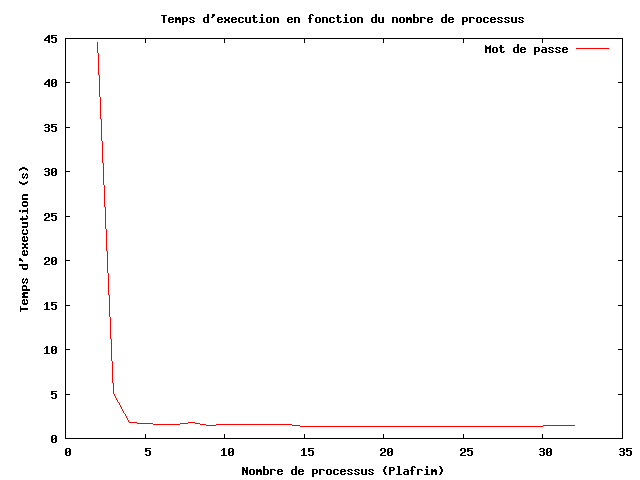
\includegraphics[width=0.8\textwidth]{1_graph_procs}
\caption{Résultats obtenus sur Plafrim}
\label{fig:graph_procs}
\end{figure}



\section*{Introduction} % (fold)
\addcontentsline{toc}{section}{Introduction}
\label{sec:introduction}

Le projet est opérationnel et donne des performances raisonnables. Nous regrettons simplement de ne pas avoir des performances plus précises en fonction de l'influence du nombre de \emph{threads} ou de la taille des blocs de tâches, nous pensons toutefois que ce n'était pas le but de ce projet. Des améliorations possibles ont été évoquées -- comme la génération des intervalles -- mais nous avons trouvé cela trop difficile à mettre en place.


%% \input{X-Conclusion.tex}


\end{document}
